\documentclass[degree=doctor]{ahuthesis}
  % 学位 degree:
  %  doctor | master | bachelor | postdoc
  % 学位类型 degree-type:
  %  academic (默认) | professional
  % 语言 language
  %  chinese (默认) | english
  % 字体库 fontset
  %  windows | mac | ubuntu
  % 超链接的彩色模式: 
  % nocolor
  % 建议终版使用 Windows 平台的字体编译

% 论文基本配置, 加载宏包等全局配置
% !TeX root = ./ahuthesis-example.tex

% 论文基本信息配置

\ahusetup{
  %******************************
  % 注意:
  %   1. 配置里面不要出现空行
  %   2. 不需要的配置信息可以删除
  %   3. 建议先阅读文档中所有关于选项的说明
  %******************************
  %
  % 输出格式
  %   选择打印版 (print) 或用于提交的电子版 (electronic), 前者会插入空白页以便直接双面打印
  %
  output = print,
  %
  % 标题 (可使用“\\”命令手动控制换行)
  %
  title  = {安徽大学学位论文 \LaTeX{} 模板使用示例文档 v\version},
  title* = {An Introduction to \LaTeX{} Thesis Template of Anhui
            University v\version},
  %
  %%%%%%%%%%%%%%%%%%%%%%%%%%% 博士学位论文信息填写 %%%%%%%%%%%%%%%%%%%%%%%%%%%
  clc              = {O157.5},                % 中图分类号
  degree-category  = {理学博士},
  degree-category* = {Doctor of Philosophy},
  %
  department = {数学科学学院},                 % 培养单位(填写所属院系的全名)
  discipline  = {数学},                       % 一级学科(中文)
  discipline* = {Mathematics},               % 一级学科(英文)
  sub-discipline = {基础数学},                % 二级学科
  author  = {作者姓名},                       % 作者姓名(中文)
  author* = {Name},                          % 作者姓名(英文)
  student-id = {A20614045},                  % 学号
  supervisor  = {xxx},                       % 指导教师(中文姓名和职称之间以英文逗号“,”分开, 下同)
  supervisor* = {xxx},
  professional-rank = {教授},                % 指导教师的职称
  % 提名页信息填写
  start-date = {2015-09-01},                % 学习开始日期
  end-date   = {2019-02-01},                % 学习结束日期
  date       = {2019-06-01},                % 论文提交日期
  defense-date = {2019-05-01},              % 论文答辩日期
  % 是否在中文封面后的空白页生成书脊(默认 false)
  include-spine = true,
  spine-date = {2025},
  %
  % 
  %%%%%%%%%%%%%%%%%%%%%%%%%%% 硕士信息填写 %%%%%%%%%%%%%%%%%%%%%%%%%%%
  % clc              = {O157.5},                % 中图分类号
  % degree-category  = {理学硕士},
  % degree-category* = {Doctor of Philosophy},
  % %
  % department = {数学科学学院},                 % 培养单位(填写所属院系的全名)
  % discipline  = {数学},                       % 一级学科(中文)
  % discipline* = {Mathematics},               % 一级学科(英文)
  % sub-discipline = {基础数学},                % 二级学科
  % author  = {作者姓名},                       % 作者姓名(中文)
  % author* = {Name},                      % 作者姓名(英文)
  % student-id = {A20614045},                  % 学号
  % supervisor  = {xxx},                       % 指导教师(中文姓名和职称之间以英文逗号“,”分开, 下同)
  % supervisor* = {xxx},
  % professional-rank = {教授},                % 指导教师的职称
  % % 提名页信息填写
  % start-date = {2015-09-01},                % 学习开始日期
  % end-date   = {2019-02-01},                % 学习结束日期
  % date       = {2019-06-01},                % 论文提交日期
  % defense-date = {2019-05-01},              % 论文答辩日期
  % % 是否在中文封面后的空白页生成书脊(默认 false)
  % include-spine = true,
  % spine-date = {2025},
  %
  %
  %%%%%%%%%%%%%%%%%%%%%%%%%%% 博士后出站报告信息填写 %%%%%%%%%%%%%%%%%%%%%%%%%%%
  %
  % clc            = {O157.5},           % 中图分类号
  % udc            = {UDC},
  % id             = {编号},
  % discipline     = {一级学科},          % 流动站(一级学科)名称
  % sub-discipline = {二级学科},          % 专业(二级学科)名称
  % start-date     = {2011-07-01},       % 研究工作起始时间
}
  %
  % 
%%%%%%%%%%%%%%%%%%%%%%%%%%% 载入所需的宏包 %%%%%%%%%%%%%%%%%%%%%%%%%%%
% 定理类环境宏包
\usepackage{amsthm}
% 也可以使用 ntheorem
% \usepackage[amsmath,thmmarks,hyperref]{ntheorem}

\ahusetup{
  % 数学字体
  math-font  = newcm,  % xits | newcm
  cite-style = super
}

% 表格加脚注
\usepackage{threeparttable}

% 跨页表格
\usepackage{longtable}

% 算法
\usepackage{algorithm}
\usepackage{algorithmic}

% 量和单位
\usepackage{siunitx}

% 参考文献使用 BibTeX + natbib 宏包
% 顺序编码制
\usepackage[sort]{natbib}
\bibliographystyle{ahuthesis-numeric}

% 著者-出版年制
% \usepackage{natbib}
% \bibliographystyle{ahuthesis-author-year}

% 定义所有的图片文件在 figures 子目录下
\graphicspath{{figures/}}

% 数学命令
\makeatletter
\newcommand\dif{%  % 微分符号
  \mathop{}\!\mathrm{d}%
}
\makeatother

% hyperref 宏包在最后调用
\usepackage{hyperref}

\begin{document}
% 封面 (博士/硕士的封面是否显示. 如果不需要封面可将此命令注释掉)
\makecover
% 封面
\maketitle

% 使用授权的说明
\copyrightpage
% 将签字扫描后授权文件 scan-copyright.pdf 替换原始页面
% \copyrightpage[file=scan-copyright.pdf]

\frontmatter
% !TeX root = ../ahuthesis-example.tex

% 中英文摘要和关键字

\begin{abstract}
论文的摘要是对论文研究内容和成果的高度概括. 摘要应对论文所研究的问题
及其研究目的进行描述, 对研究方法和过程进行简单介绍, 对研究成果和所得
结论进行概括. 摘要应具有独立性和自明性, 其内容应包含与论文全文同等量
的主要信息. 使读者即使不阅读全文, 通过摘要就能了解论文的总体内容和主要成果.

论文摘要的书写应力求精确、简明. 切忌写成对论文书写内容进行提要的形式.

关键词是为了文献标引工作、用以表示全文主要内容信息的单词或术语.

% 关键词用“英文逗号”分隔,输出时会自动处理为正确的分隔符
\ahusetup{
  keywords = {关键词 1, 关键词 2, 关键词 3, 关键词 4, 关键词 5},
  }
\end{abstract}

\begin{abstract*}
An abstract of a dissertation is a summary and extraction of research work and contributions.
Included in an abstract should be description of research topic and research objective, 
brief introduction to methodology and research process, and summary of conclusion and 
contributions of the research. An abstract should be characterized by independence and 
clarity and carry identical information with the dissertation. It should be such that the 
general idea and major contributions of the dissertation are conveyed without reading the dissertation.

An abstract should be concise and to the point. It is a misunderstanding to make an abstract 
an outline of the dissertation.

Keywords are terms used in a dissertation for indexing, reflecting core information of the dissertation.

% Use comma as separator when inputting
\ahusetup{
  keywords* = {keyword 1, keyword 2, keyword 3, keyword 4, keyword 5},
  }
\end{abstract*}

% 目录
\tableofcontents

% 插图和附表清单
% 本科生的插图索引和表格索引需要移至正文之后、参考文献前
% \listoffiguresandtables  % 插图和附表清单(仅限研究生)
\listoffigures           % 插图清单
\listoftables            % 附表清单

% 符号对照表
% !TeX root = ../ahuthesis-example.tex

\begin{center}
\begin{denotation}[1cm]
  \item[$\mathbb{N}$] 自然数集
  \item[$\mathbb{Q}$] 有理数集
  \item[$\mathbb{R}$] 实数集
\end{denotation}
\end{center}


% 也可以使用 nomencl 宏包, 需要在导言区
% \usepackage{nomencl}
% \makenomenclature

% 在这里输出符号说明
% \printnomenclature[3cm]

% 在正文中的任意为都可以标题
% \nomenclature{$\mathbb{N}$}{自然数集}
% \nomenclature{$\mathbb{Q}$}{有理数集}


% 正文部分
\mainmatter
% !TeX root = ../ahuthesis-example.tex

\chapter{论文的基本要求及内容}

学位论文是标明作者从事科学研究取得的创造性成果和创新见解, 并以此为内容撰写的、作
为申请学位时评审用的学术论文. 硕士学位论文应表明作者在本门学科上掌握了坚实的基础
理论和系统的专门知识, 对所研究的课题有新的见解, 并具有从事科学研究工作或独立担负
专门技术工作能力. 博士学位论文应表明作者在本门学科上掌握了坚实宽广的基础理论和系
统深入的专门知识, 在科学和专门技术上做出了创造性的成果, 并具有独立从事科学研究工
作的能力. 为提高研究生学位论文的质量, 做到学位论文在内容和格式上的统一和规范, 根
据《中华人民共和国国家标准科学技术报告、学位论文和学术论文的编写格式》(GB/T 7713.1--2006)
的规定, 特制定《安徽大学研究生撰写学位论文的规定》.


\section{论文的基本要求}

论文应立论正确、推理严谨、说明透彻、数据可靠. 论文应结构合理、层次分明、叙述准确、
文字简练、文图规范. 对于涉及作者创新性工作和研究特点的内容应重点论述, 做到数据或
实例丰富、分析全面深入. 文中引用的文献资料必须注明来源, 使用的计量单位、绘图规范
应符合国家标准. 论文的学术水平应满足《安徽大学申请博士、硕士学位学术成果基本要求》的要求.


\section{论文内容}

包括: 选题的背景、依据及意义; 文献及相关研究综述、研究及设计方案、试验方法、装置和试验结果;
理论的证明、分析和结论;重要的计算、数据、图表、曲线及相关分析; 必要的附录、相关的参考文献目录等.

对于合作完成的项目, 论文的内容应侧重本人的研究工作. 论文中有关与指导教师或他人共同
研究、试验的部分以及引用他人研究成果的部分都要明确说明.


\section{论文的书写规范与打印要求}

\subsection{论文的文字}

除英文封面、英文摘要外, 研究生学位论文的其余部分都应该用中文撰写, 以下两种情况除外:

(1) 留学生学位论文的目录、正文和致谢等可用英文撰写; 但封面、题名页、独创性声明和使用授权书应用中文撰写, 摘要应中英文对照撰写.

(2) 外语专业的学位论文的目录、正文和致谢等应用所学专业相应的语言撰写; 但封面、题名页、独创性声明和使用授权书应用中文撰写, 
摘要应使用中文和所学专业相应的语言对照撰写. 

\subsection{论文的书写}

学位论文一律由本人在计算机上输入、编排并打印在标准 A4 纸上, 封面(中、英文)、题名页、独创性声明和使用授权书采用单面印刷,
从中文摘要开始采用双面印刷(总页数少于 100 页的学位论文, 为了制作书脊的需要, 可以采用单面印刷, 单面印刷可以允许用 
$210\times 297$mm, 70g 的纸张). 应该便于阅读、复制和拍摄缩微制品.


\section{论文的主要结构及装订顺序}

学位论文一般应由 $12$ 个部分组成, 装订顺序依次为:

(1) 封面(中、英文)	

(2) 题名页	

(3) 独创性声明和使用授权书	

(4) 中文摘要	

(5) 英文摘要	

(6) 目录

(7) 图表清单及主要符号表(根据具体情况可省略)	

(8) 主体部分

(9) 参考文献

(10) 附录

(11) 攻读博士学位期间参与的科研项目和取得的研究成果/攻读硕士学位期间参与的科研项目和取得的学术成果

(12) 致谢
% !TeX root = ../ahuthesis-example.tex

\chapter{图表示例}

\section{插图}

图片通常在 \env{figure} 环境中使用 \cs{includegraphics} 插入, 如图~\ref{fig:example} 的源代码.
建议矢量图片使用 PDF 格式, 比如数据可视化的绘图; 照片应使用 JPG 格式; 其他的栅格图应使用无损的 PNG 格式.
注意, EPS 格式已经过时.

\begin{figure}
  \centering
  
\includegraphics[width=0.5\linewidth]{ahulogo.pdf}
  \caption{示例图片标题}
  \label{fig:example}
\end{figure}

若图或表中有附注, 采用英文小写字母顺序编号, 附注写在图或表的下方.
国外的期刊习惯将图表的标题和说明文字写成一段, 需要改写为标题只含图表的名称,
其他说明文字以注释方式写在图表下方或者写在正文中.

如果一个图由两个或两个以上分图组成时, 各分图分别以 (a), (b), (c) ... 作为图序, 并须有分图题.
推荐使用 \pkg{subcaption} 宏包来处理, 比如图~\ref{fig:subfig-a} 和图~\ref{fig:subfig-b}.

\begin{figure}
  \centering
  \subcaptionbox{分图 A\label{fig:subfig-a}}
    {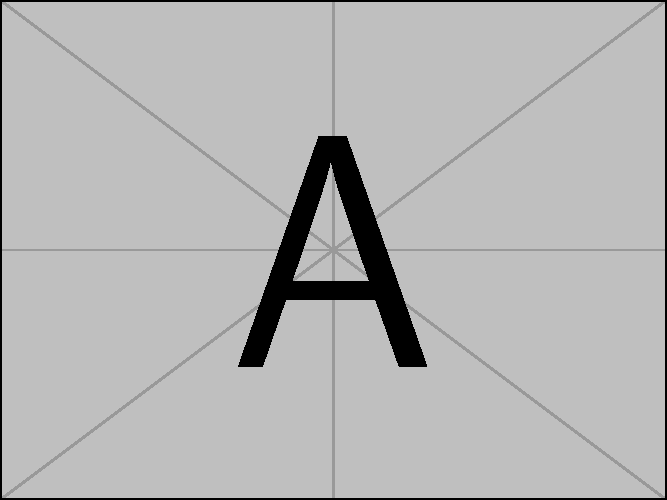
\includegraphics[width=0.35\linewidth]{example-image-a.pdf}}
  \subcaptionbox{分图 B\label{fig:subfig-b}}
    {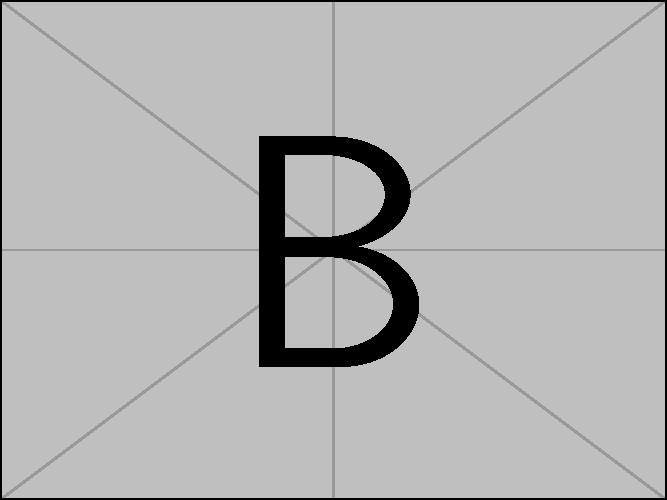
\includegraphics[width=0.35\linewidth]{example-image-b.pdf}}
  \caption{多个分图的示例}
  \label{fig:multi-image}
\end{figure}


\section{表格}

表应具有自明性, 为使表格简洁易读, 尽可能采用三线表, 如表~\ref{tab:three-line}.
三条线可以使用 \pkg{booktabs} 宏包提供的命令生成.

\begin{table}
  \centering
  \caption{三线表示例}
  \begin{tabular}{ll}
    \toprule
    文件名          & 描述                         \\
    \midrule
    ahuthesis.dtx   & 模板的源文件,包括文档和注释 \\
    ahuthesis.cls   & 模板文件                     \\
    ahuthesis-*.bst & BibTeX 参考文献表样式文件    \\
    \bottomrule
  \end{tabular}
  \label{tab:three-line}
\end{table}

表格如果有附注, 尤其是需要在表格中进行标注时, 可以使用 \pkg{threeparttable} 宏包.
附注各项的序号一律用“附注 + 阿拉伯数字 + 冒号”.

\begin{table}
  \centering
  \begin{threeparttable}[c]
    \caption{带附注的表格示例}
    \label{tab:three-part-table}
    \begin{tabular}{ll}
      \toprule
      文件名                 & 描述                         \\
      \midrule
      ahuthesis.dtx\tnote{1} & 模板的源文件,包括文档和注释 \\
      ahuthesis.cls\tnote{2} & 模板文件                     \\
      ahuthesis-*.bst        & BibTeX 参考文献表样式文件    \\
      \bottomrule
    \end{tabular}
    \begin{tablenotes}[online]
      \item[附注 1:] 可以通过 xelatex 编译生成模板的使用说明文档;
        使用 xetex 编译 \file{thuthesis.ins} 时则会从 \file{.dtx} 中去除掉文档和注释, 得到精简的 \file{.cls} 文件.
      \item[附注 2:] 更新模板时, 一定要记得编译生成 \file{.cls} 文件, 否则编译论文时载入的依然是旧版的模板.
    \end{tablenotes}
  \end{threeparttable}
\end{table}

如某个表需要转页接排,可以使用 \pkg{longtable} 宏包.


\section{算法}

算法环境可以使用 \pkg{algorithms} 或者 \pkg{algorithm2e} 宏包.

\renewcommand{\algorithmicrequire}{\textbf{输入:}\unskip}
\renewcommand{\algorithmicensure}{\textbf{输出:}\unskip}

\begin{algorithm}
  \caption{Calculate $y = x^n$}
  \label{alg1}
  \small
  \begin{algorithmic}
    \REQUIRE $n \geq 0$
    \ENSURE $y = x^n$

    \STATE $y \leftarrow 1$
    \STATE $X \leftarrow x$
    \STATE $N \leftarrow n$

    \WHILE{$N \neq 0$}
      \IF{$N$ is even}
        \STATE $X \leftarrow X \times X$
        \STATE $N \leftarrow N / 2$
      \ELSE[$N$ is odd]
        \STATE $y \leftarrow y \times X$
        \STATE $N \leftarrow N - 1$
      \ENDIF
    \ENDWHILE
  \end{algorithmic}
\end{algorithm}
% !TeX root = ../ahuthesis-example.tex

\chapter{数学符号和公式}

\section{数学符号}

中文论文的数学符号默认遵循 GB/T 3102.11--1993《物理科学和技术中使用的数学符号》
\footnote{原 GB 3102.11—1993, 自 2017 年 3 月 23 日起, 该标准转为推荐性标准.}.
具体地来说主要有以下差异:
\begin{enumerate}
  \item 实部 $\Re$ 和虚部 $\Im$ 的字体使用罗马体.
\end{enumerate}

另外国标还有一些与 AMS 不同的符号使用习惯, 需要用户在写作时进行处理:
\begin{enumerate}
  \item 数学常数和特殊函数名用正体, 如
    \begin{equation*}
      \uppi = 3.14\dots; \quad
      \symup{i}^2 = -1; \quad
      \symup{e} = \lim_{n \to \infty} \left( 1 + \frac{1}{n} \right)^n.
    \end{equation*}
  \item 微分号使用正体, 比如 $\dif y / \dif x$.
  \item 自然对数用 $\ln x$ 不用 $\log x$.
\end{enumerate}

关于量和单位推荐使用 \pkg{siunitx} 宏包, 可以方便地处理希腊字母以及数字与单位之间的空白, 比如:
\SI{6.4e6}{m}, \SI{9}{\micro\meter}, \si{kg.m.s^{-1}}, \SIrange{10}{20}{\degreeCelsius}.


\section{数学公式}

数学公式可以使用 \env{equation} 和 \env{equation*} 环境。
注意数学公式的引用应前后带括号, 通常使用 \cs{eqref} 命令, 比如式 \eqref{eq:example}.
\begin{equation}
  \frac{1}{2 \uppi \symup{i}} \int_\gamma f = \sum_{k=1}^m n(\gamma; a_k) \mathscr{R}(f; a_k).
  \label{eq:example}
\end{equation}

多行公式尽可能在“=”处对齐, 推荐使用 \env{align} 环境.
\begin{align}
  a & = b + c + d + e \\
    & = f + g
\end{align}


\section{数学定理}

定理环境的格式可以使用 \pkg{amsthm} 或者 \pkg{ntheorem} 宏包配置.
用户在导言区载入这两者之一后, 模板会自动配置 \env{theorem}, \env{proof} 等环境.

\begin{theorem}[Lindeberg--Lévy 中心极限定理]
  设随机变量 $X_1, X_2, \dots, X_n$ 独立同分布, 且具有期望 $\mu$ 和有限的方差 $\sigma^2 \ne 0$,
  记 $\bar{X}_n = \frac{1}{n} \sum_{i+1}^n X_i$,则
  \begin{equation}
    \lim_{n \to \infty} P \left(\frac{\sqrt{n} \left( \bar{X}_n - \mu \right)}{\sigma} \le z \right) = \Phi(z),
  \end{equation}
  其中 $\Phi(z)$ 是标准正态分布的分布函数。
\end{theorem}
\begin{proof}
  Trivial.
\end{proof}

同时模板还提供了 \env{assumption}、\env{definition}、\env{proposition}、
\env{lemma}、\env{theorem}、\env{axiom}、\env{corollary}、\env{exercise}、
\env{example}、\env{remar}、\env{problem}、\env{conjecture} 这些相关的环境.


% 其他部分
\backmatter

% 参考文献
\bibliography{refs}        % 参考文献使用 BibTeX 编译

% 附录
\appendix
% !TeX root = ../ahuthesis-example.tex

\chapter{补充内容}

附录是与论文内容密切相关、但编入正文又影响整篇论文编排的条理和逻辑性的资料, 例如某些重要的数据表格、
计算程序、统计表等, 是论文主体的补充内容, 可根据需要设置.

附录中的图、表、数学表达式、参考文献等另行编序号, 与正文分开, 一律用阿拉伯数字编码,
但在数码前冠以附录的序号, 例如“图~\ref{fig:appendix-figure}”,
“表~\ref{tab:appendix-table}”, “式 \eqref{eq:appendix-equation}”等.


\section{插图}

\begin{figure}
  \centering
  
\includegraphics[width=0.6\linewidth]{ahulogo.pdf}
  \caption{附录中的图片示例}
  \label{fig:appendix-figure}
\end{figure}


\section{表格}

\begin{table}
  \centering
  \caption{附录中的表格示例}
  \begin{tabular}{ll}
    \toprule
    文件名          & 描述                         \\
    \midrule
    ahuthesis.dtx   & 模板的源文件, 包括文档和注释 \\
    ahuthesis.cls   & 模板文件                     \\
    ahuthesis-*.bst & BibTeX 参考文献表样式文件    \\
    \bottomrule
  \end{tabular}
  \label{tab:appendix-table}
\end{table}


\section{数学表达式}

\begin{equation}
  \frac{1}{2 \uppi \symup{i}} \int_\gamma f = \sum_{k=1}^m n(\gamma; a_k) \mathscr{R}(f; a_k)
  \label{eq:appendix-equation}
\end{equation}
% 致谢
% !TeX root = ../ahuthesis-example.tex

\begin{acknowledgements}
这里撰写致谢内容.
\end{acknowledgements}

% 在学期间完成的相关学术成果
% !TeX root = ../ahuthesis-example.tex

\begin{resume}

\section*{个人简历}

xxxx 年 xx 月出生于 xx 省 xx 县.

xxxx 年 09 月考入 xx 大学数学科学学院; xxxx 年 07 月本科毕业并获得理学学士学位.

xxxx 年 09 月进入 xx 大学攻读 xx 博士至今.


\section*{在学期间完成的相关学术成果}
\subsection*{学术论文}

\begin{achievements}
\item Lele Liu, Extremal spectral radius of nonregular graphs with prescribed maximum degree, 
\emph{Journal of Combinatorial Theory, Series B}, 169: 430--479, 2024.

\item Lele Liu, Graph limits and spectral extremal problems for graphs, 
\emph{SIAM Journal on Discrete Mathematics}, 38(1): 590--608, 2024.
\end{achievements}

\end{resume}

\end{document}
